\begin{figure}[!tb]
\begin{center}
\begin{tikzpicture}[]
\fill (0,0) node[inner sep=1pt] (A) {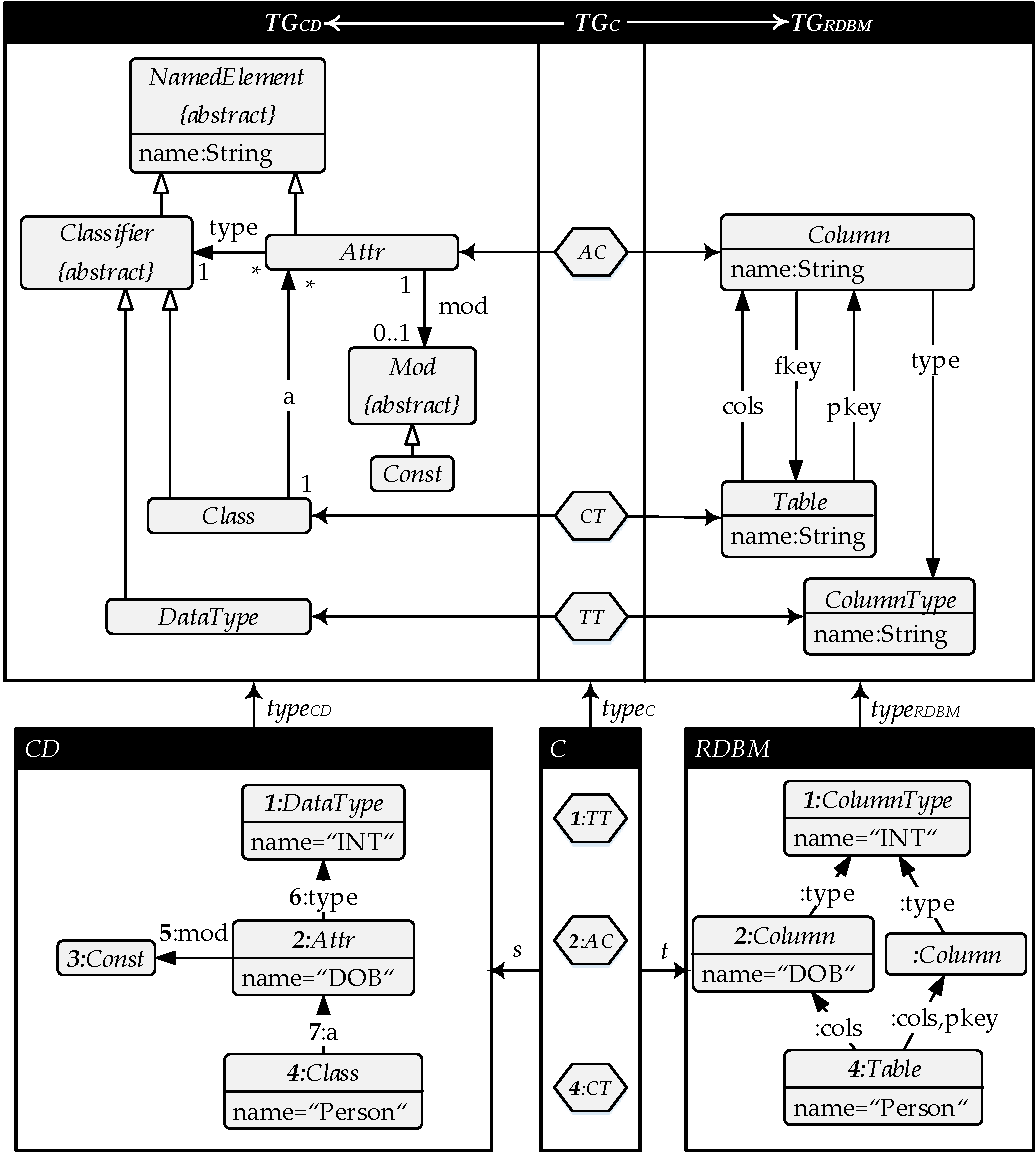
\includegraphics[width=.9\textwidth]{img/gen_intro/atg.pdf}};
%\fill (-2.5,7.55) node[inner sep=1pt] (B) {\textcolor{white}{$(\TG_\CD \gets \Corr \to \TG_\RDBM)$}};
\end{tikzpicture}
\end{center}
\caption{Attributed Triple Type Graph $(\TG_\CD \gets \TG_C \to \TG_\RDBM)$ (top) \& Typed Attributed Triple Graph $(\CD \transB{s} C \trans{t} \RDBM)$ (bottom)}
\label{fig:sec-gt-graphs:atg}
\label{fig:mm}
\end{figure}

We assume that (visual) models are represented by graphs (cf. \cref{sec-gen-intro-gratrafo}).
A plain graph consists of nodes (vertices) and edges between nodes.
An edge links a source node with a target node.
The presented notion of graphs allows parallel edges between two nodes and edge loops.
A morphism $f\colon G_1 \to G_2$ from a graph $G_1$ to a graph $G_2$ is a mapping from nodes and edges in $G_1$ to nodes and edges in $G_2$ such that the structure of $G_1$ is preserved, i.e, the source (target) node of each edge $e$ in $G_1$ is mapped to the source (target) node of edge $f(e)$ in $G_2$.

\begin{definition}[Graph and Graph Morphism (Def. 2.1 in \cite{FAGT2})]
A \emph{graph}\index{graph} $G=(V_G,E_G,s_G\colon E_G \to V_G,t_G\colon E_G \to V_G)$ consists of a set of nodes $V_G$, a set of edges $E_G$ and two functions $s_G,t_G$ that map the source node (via $s_G$) and target node (via $t_G$) to each edge.
A \emph{graph morphism}\index{graph!morphism} $f\colon G_1 \to G_2$ from $G_1$ to $G_2$ with $f=(f_V,f_E)$ consists of two functions $f_V\colon V_{G_1} \to V_{G_2},f_E\colon E_{G_1} \to E_{G_2}$ such that $s_{G_2} \circ f_E=f_V \circ s_{G_1}$ and $t_{G_2} \circ f_E=f_V \circ t_{G_1}$.
\envEndMarker
\end{definition}

A typed graph is a plain graph $G$ together with a graph morphism from $G$ to a distinguished type graph $\TG$ that defines the typing of each node and edge in $G$ - We say that $G$ is typed over $\TG$.
Therefore, a type graph is part of the meta-model for a given domain and defines the concepts (node types) for the domain and their interrelationships (edge types) that can be used in graphs as models in the domain (cf. \cref{sec-gen-intro-mt,fig:sec-gen-intro-mt:meta}).
A typed graph morphism between two typed graphs is a graph morphism that additionally preserves the typing.

\parpic[r][r]{
$
\SelectTips{cm}{}
     \xymatrix@R-3.3ex@C-2ex{
     G_1 \ar[rr]^{f} \ar[dddr]_{\type_{G_1}} & \ar@{}[dd]|{(=)} & G_2 \ar[dddl]^{\type_{G_2}} \\
     & & \\
     & & \\
     & \TG & \\
     }
$
}
\vspace{-1.5ex}

\begin{definition}[Typed Graph and Typed Graph Morphism (Def. 2.2 in \cite{FAGT2})]
\label{def:sec-gt-graphs:typed_graphs}
Given a distinguished graph $\TG$ as the type graph.
A \emph{typed graph $G^\T=(G,\type_G\colon G \to \TG)$ over $\TG$}\index{graph!typed} is given by a graph $G$ and a graph morphism $\type_G$ from $G$ to $\TG$.
A \emph{typed graph morphism}\index{graph!morphism!typed} $f\colon G^\T_1 \to G^\T_2$ is a graph morphism $f\colon G_1 \to G_2$ such that $\type_{G_2} \circ f=\type_{G_1}$.
\envEndMarker
\end{definition}

Attributed graphs are defined based on the notion of E-graphs that allow the attribution of edges and nodes.
The set of possible attribute values is defined by an algebra.
For an introduction to algebraic signatures and algebras we refer to \cite{Ehrig:2006:FAG:1121741}.

\parpic[r][r]{
$
\SelectTips{cm}{}
     \xymatrix@R-3.3ex@C-2ex{
     & E^G_G \ar@/^/[rr]^{s^G_G} \ar@/_/[rr]_{t^G_G} & & V^G_G & \\
     & & & & \\
     & & & & \\
     E^G_{EA} \ar[uuur]^{s^G_{EA}} \ar[rr]^{t^G_{EA}} & & V^G_D & & E^G_{NA} \ar[uuul]_{s^G_{NA}} \ar[ll]_{t^G_{NA}} \\
     }
$
}
\vspace{-1.5ex}

\begin{definition}[Attributed Graph and Attributed Graph Morphism (Def. 2.4 in \cite{FAGT2})]
\label{def:sec-gt-graphs:agraphs}
An \emph{E-graph}\index{graph!E-graph} $G^\EE=(V_G^G,V_D^G,E_G^G,E_{NA}^G,E_{EA}^G,(s_i^G,t_i^G)_{i \in \{G,NA,EA\}})$ with graph nodes $V_G^G$, data nodes $V_D^G$, graph edges $E_G^G$, node attribute edges $E_{NA}^G$, edge attribute edges $E_{EA}^G$ and source and target functions $s_i^G,t_i^G$ with signatures as defined on the right.
An \emph{E-graph morphism}\index{graph!morphism!E-graph} $f\colon G^\EE_1 \to G^\EE_2$ with $f=((f_{V_i}\colon V_i^{G_1} \to V_i^{G_2})_{i \in \{G,D\}}, (f_{E_j}\colon E_j^{G_1} \to E_j^{G_2})_{j \in \{G,NA,EA\}})$ is a pair of tuples of functions $f_{V_i}$ for mapping nodes and functions $f_{E_j}$ for mapping edges from $G^\EE_1$ to $G^\EE_2$ such that $f$ commutes with all source and target functions.
Given a data signature $\DSIG=(S,\OP)$, then an \emph{attributed graph over $\DSIG$}\index{graph!attributed} is given by $G=(G^\EE,D_G)$ with $G^\EE$ being an E-graph and $D_G$ being a $\DSIG$-algebra such that $\dot{\cup}_{s \in S}(D_{G,s})=V^G_D$.
Given attributed graphs $G_1$ and $G_2$ over common $\DSIG$, then an \emph{attributed graph morphism}\index{graph!morphism!attributed} $f\colon G_1 \to G_2$ from $G_1$ to $G_2$ with $f=(f_G,f_D)$ is a pair of an E-graph morphism $f_G\colon G^\EE_1 \to G^\EE_2$ and an algebra homomorphism $f_D\colon D_{G_1} \to D_{G_2}$ such that $f_{G,V_D}(x)=f_{D,s}(x)$ for all $x \in D_{G_1,s},s \in S$.
\index{graph!attributed!graph part}\index{graph!attributed!data part}With $(V^G_G,(E^G_X)_{X \in \{G,NA,EA\}})$ we refer to the (structural) graph part of attributed graph $G$ and distinguish it from its data part $(V^G_D,D_G)$.
\index{graph!morphism!attributed -- graph part}\index{graph!morphism!attributed -- data part}With $f_S=(f_{G,V_G},f_{G,E_G},f_{G,E_{NA}},f_{G,E_{EA}})$ we refer to the (structural) graph part of attributed graph morphism $f$ and distinguish it from its data part $f_D$.
\envEndMarker
\end{definition}

Typed and attributed graphs (morphisms) are combined to typed attributed graphs (morphisms).

\begin{definition}[Typed Attributed Graph and Morphism (Def. 2.5 in \cite{FAGT2})]
\label{def:sec-gt-graphs:typed_attr_graphs}
Given a distinguished attributed graph $\ATG=(\TG,Z)$ as attributed type graph with $Z$ being the final $\DSIG$-algebra.
The final $\DSIG$-algebra \index{final $\DSIG$-algebra}contains exactly one element in each carrier set.
A \emph{typed attributed graph \index{graph!typed \& attributed} $G^\T=(G,\type_G\colon G \to \ATG)$ over $\ATG$} is given by an attributed graph $G$ over $\DSIG$ and an attributed graph morphism $\type_G$ from $G$ to $\ATG$.
Given typed attributed graphs $G^\T_1$ and $G^\T_2$ over common $\ATG$, then a \emph{typed attributed graph morphism}\index{graph!morphism!typed \& attributed} $f\colon G^\T_1 \to G^\T_2$ is an attributed graph morphism $f\colon G_1 \to G_2$ such that $\type_{G_2} \circ f=\type_{G_1}$.
\envEndMarker
\end{definition}

\begin{remark}[Typed Attributed Graphs with Node Type Inheritance]
\label{rem:sec-gt-graphs:inheritance}
Typed attributed graphs and morphisms are extended to typed attributed graphs and morphisms with node type inheritance.
Therefore, the type graph is extended with an additional inheritance relation between nodes that defines which nodes in the type graph inherit from which other nodes.
Furthermore, nodes in the type graph can be explicitly marked as abstract, i.e., abstract nodes cannot be directly used as concrete types for nodes in graphs that are typed over this type graph.
A node \code{A} that inherits from a node \code{B} shares all node attributes as well as incoming and outgoing edges of \code{B} with \code{B}.
If node \code{A} inherits from node \code{B}, then \code{A} is called the sub-node (sub-type) of \code{B} whereas \code{B} is called the super-node (super-type) of \code{A}.
A morphism between two typed attributed graphs $G_1$ and $G_2$ with node type inheritance may refine the types of nodes from $G_1$ to $G_2$ by mapping nodes in $G_1$ of super-type \code{B} to nodes in $G_2$ of sub-type \code{A}.
Basically beside abstract nodes, typed graphs with node type inheritance do not lead to additional expressiveness in comparison to graphs without node type inheritance, since, the type graph with inheritance can most widely be flattened to a type graph without inheritance information by duplicating edges and attributes from super-nodes to sub-nodes (cf. Def. 6 in \cite{DBLP:journals/tcs/GolasLEO12}). 
However, type graphs with inheritance allow a more compact notation in comparison to their flattened versions (cf. Figs. 1 and 4 in \cite{DBLP:journals/tcs/GolasLEO12}).
We allow inheritance in type graphs and refer to \cite{DBLP:journals/tcs/GolasLEO12} for technical details.
\envEndMarker
\end{remark}

\begin{example}[Attributed Type Graph \& Typed Attributed Graph]
\label{ex:sec-gt-graph:type_graph}
\cref{fig:sec-gt-graphs:atg} depicts attributed type graphs $\TG_\CD$ and $\TG_\RDBM$ for class diagrams ($\CD$) and relational database models ($\RDBM$).
Both type graphs are part of the meta-models for the domains of CDs and RDBMs.
Class diagrams may contain several \code{Class}es, each with a set of class \code{Attr}ibutes that are assigned via \code{a} edges to the class.
Furthermore, each attribute is \code{type}d by a \code{Classifier}.
By node type inheritance, classifiers are classes or other \code{DataType}s.
Furthermore by node type inheritance, each class, attribute and data type is a \code{NamedElement} and therefore has a specific \code{name} of type \code{String}.
Moreover, attributes may have a \code{Mod}ifier \code{Const}ant which declares that the attribute value does not change.
Note that nodes \code{NamedElement}s, \code{Classifier}s and \code{Mod}ifiers are marked as \code{abstract} and therefore, they cannot be directly used as concrete types in class diagrams but their sub-nodes (sub-types).

Relational database models may contain several \code{Table}s.
A table has a \code{name} of type \code{String} and may have several \code{Column}s assigned via \code{cols} edges where one column may contain the primary keys of the rows of the table (edge \code{pkey}) or columns may refer to other tables by foreign keys (\code{fkey}).
Furthermore, each column has a specific \code{name} of type \code{String} and is of a specific \code{type}.
Analogously, each column type has a \code{name} of type \code{String}.

The multiplicity constraints on the edges in type graph $\TG_\CD$ are expressed by graph constraints in \cref{sec-gt-gc,ex:sec-gc-gc:gc_UML_CD} and complete the meta-model for the domain of UML class diagrams.

Typed attributed graph $\CD$ ($\RDBM$) is a class diagram (relational database model) typed over type graph $\TG_\CD$ ($\TG_\RDBM$) via morphism $\type_\CD$ ($\type_{\RDBM}$).
The class diagram $\CD$ contains a class of name \code{``Person''} together with a class attributes \code{``DOB''} (date of birth) of type \code{``INT''}.
Furthermore, attribute \code{``DOB''} is equipped with modifier \code{Const} (constant).
For typing, node \code{2} in $\CD$ is mapped to node \code{Attr} in $\TG_\CD$ along morphism $\type_\CD$.
All other nodes, edges and node attributes in $\CD$ are mapped analogously.
The formal notation of graph $\CD$ is given below:
\paragraph*{}
$\CD=(\underline{\CD},\type_{\underline{\CD}}\colon \underline{\CD} \to \TG_\CD)$ where $\underline{\CD}=(\underline{\CD}^E=(V_G^{\underline{\CD}},V_D^{\underline{\CD}},E_G^{\underline{\CD}},E_{NA}^{\underline{\CD}},E_{EA}^{\underline{\CD}},$ $(s_i^{\underline{\CD}},t_i^{\underline{\CD}})_{i \in \{G,NA,EA\}}),D_{\underline{\CD}})$ with 
\newline
$V_G^{\underline{\CD}}=\{1,2,3,4\},$
\newline
$V_D^{\underline{\CD}}=D_{\underline{\CD},String},$
\newline
$E_G^{\underline{\CD}}=\{5,6,7\},$
\newline
$E_{NA}^{\underline{\CD}}=\{a,b,c\},$
\newline
$E_{EA}^{\underline{\CD}}=\{\},$
\newline
$s_G^{\underline{\CD}}=(5 \mapsto 2,6 \mapsto 2,7 \mapsto 4),$
\newline
$t_G^{\underline{\CD}}=(5 \mapsto 3,6 \mapsto 1,7 \mapsto 2),$
\newline
$s_{NA}^{\underline{\CD}}=(a \mapsto 1,b \mapsto 2, c \mapsto 4),$
\newline
$t_{NA}^{\underline{\CD}}=(a \mapsto ``INT'',b \mapsto ``DOB'',c \mapsto ``Person''),$
\newline
$s_{EA}^{\underline{\CD}}=t_{EA}^{\underline{\CD}}=\varnothing,$
\newline
$D_{\underline{\CD}}=(D_{\underline{\CD},String}=\{w^* \mid w \in \{a..z,A..Z\}\},OP_{D_{\underline{\CD}}}=\varnothing)$ being a $\DSIG$-algebra for algebraic data signature $\DSIG=(S=\{String\},OP=\varnothing),$ and
\newline
$\type_{\underline{\CD}}=(\type_{\underline{\CD},G}=(\type_{\underline{\CD},V_G},\type_{\underline{\CD},V_D},\type_{\underline{\CD},E_G},\type_{\underline{\CD},E_{NA}},\type_{\underline{\CD},E_{EA}}),\type_{\underline{\CD},D}\colon D_{\underline{\CD}} \to D_{\TG_\CD})$ being the type morphism with
\newline
$\type_{\underline{\CD},V_G}=(1 \mapsto DataType,2 \mapsto Attr,3 \mapsto Const,4 \mapsto Class),$
\newline
$\type_{\underline{\CD},V_D}(x)=\type_{\underline{\CD},D,String}(x),\forall x \in D_{\underline{\CD},String},$
\newline
$\type_{\underline{\CD},E_G}=(5 \mapsto mod,6 \mapsto type,7 \mapsto a),$
\newline
$\type_{\underline{\CD},E_{NA}}=(a,b,c \mapsto name),$
\newline
$\type_{\underline{\CD},E_{EA}}=\varnothing,$ and
\newline
$\type_{\underline{\CD},D,String}(x)=String,\forall x \in D_{\underline{\CD},String}$ for final $\DSIG$-algebra $D_{\TG_\CD}=(D_{\TG_\CD,String}=\{String\},OP_{D_{\TG_\CD}}=\varnothing)$ of attributed type graph $\TG_\CD$.

The relational database model $\RDBM$ contains a corresponding \code{Table}, \code{Column} and \code{ColumnType} for each \code{Class}, \code{Attr}ibute and \code{DataType} of class diagram $\CD$.
The formal notation of typed attributed graph $\RDBM$ is analogously to $\CD$.
\envEndMarker
\end{example}

\paragraph*{Visual Notation}
\label{par:sec-gt-graphs:vis}
As depicted in \cref{fig:sec-gt-graphs:atg}, nodes (edges) in typed graphs are visualised by \code{x:y} with \code{x} being the name of the node (edge) and \code{y} being the type of the node (edge).
The mapping of nodes and edges along morphisms correspond to their naming in visual notation, e.g., in visualisations of graph conditions, graph transformation rules, triple graphs and model updates (cf. \cref{sec-gt-gc,sec-gt-trafo,sec-tgg,sec-msynch-tgg}).
We omit node and edge names in visualisations if they are irrelevant and write \code{:y} instead of \code{x:y}.
Note that in formal notation of attributed graphs, node (and edge) attributes are edges and attribute values are nodes.
However, in visual notation we write \code{attr=x} for attribute \code{attr} with value \code{x} directly in the corresponding node (or edge) shape.
For an explicit visualisation of attributed graphs in E-graph notation we refer to Ex. 8.5 in \cite{Ehrig:2006:FAG:1121741}.
Although technically, a node or edge may have the same attribute several times (with possibly different attribute values), usually in practice, each node and edge has each attribute at most once such that the mapping of attributes and their values along morphisms is clear and is not explicitly visualised.